\documentclass[10pt]{beamer}
\usepackage[italian]{babel}
\usepackage[utf8]{inputenc}

\usetheme{metropolis}
\usepackage{appendixnumberbeamer}

\usepackage{booktabs}
\usepackage[scale=2]{ccicons}

\usepackage{pgfplots}
\usepgfplotslibrary{dateplot}

\usepackage{listings}
\lstset{breaklines=true}

\usepackage{xspace}
\newcommand{\themename}{\textbf{\textsc{metropolis}}\xspace}

\title{Linux Day 2017}
\subtitle{}
\date{28 Ottobre 2017}
\author{}
\institute{Latina Linux User Group}
\titlegraphic{\hfill
\includegraphics[height=1.5cm]{llg.png}}

\begin{document}

\setbeamertemplate{frame footer}{Latina Linux User Group - Linux Day 2017 - Intro}

\maketitle

\begin{frame}{Roadmap}
  \setbeamertemplate{section in toc}[sections numbered]
  \tableofcontents[hideallsubsections]
\end{frame}


\section{Com'è fatto un sistema operativo}

\begin{frame}{La composizione di un sistema operativo}

\centering 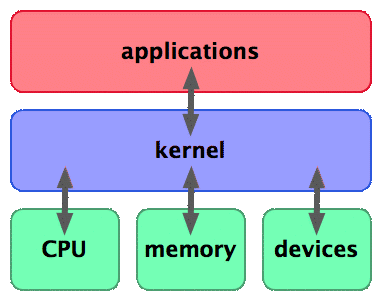
\includegraphics[scale=0.5]{kernel}

\end{frame}

\begin{frame}{La composizione di un sistema operativo (2)}

Il sistema operativo è composto da due parti principali: il \textbf{kernel} ed i programmi applicativi.

Il \textbf{kernel} è il cuore del sistema: gestisce l'hardware, la schedulazione dei processi, etc.

I \textbf{programmi applicativi} sono tutti gli altri programmi (il browser, i programmi di videoscrittura, etc)

\end{frame}

\begin{frame}{Sistemi operativi più famosi}

\begin{itemize}
\item Microsoft Windows
\item Apple macOS (già OSX)
\item GNU/Linux
\item FreeBSD/OpenBSD/NetBSD
\item Android
\end{itemize}

\end{frame}


\section{Il software libero}

\begin{frame}[fragile]{Il software proprietario}

Un software distribuito senza rilasciare il codice sorgente è detto \textbf{software proprietario}.

La licenza di un software proprietario spesso \textbf{concede in licenza} l'uso, e vieta qualsiasi altra cosa (redistribuzione, modifica, ...).

\textbf{Si acquista una licenza d'uso, non il prodotto!}

\end{frame}

\begin{frame}[fragile]{Microsoft Windows EULA}

\centering 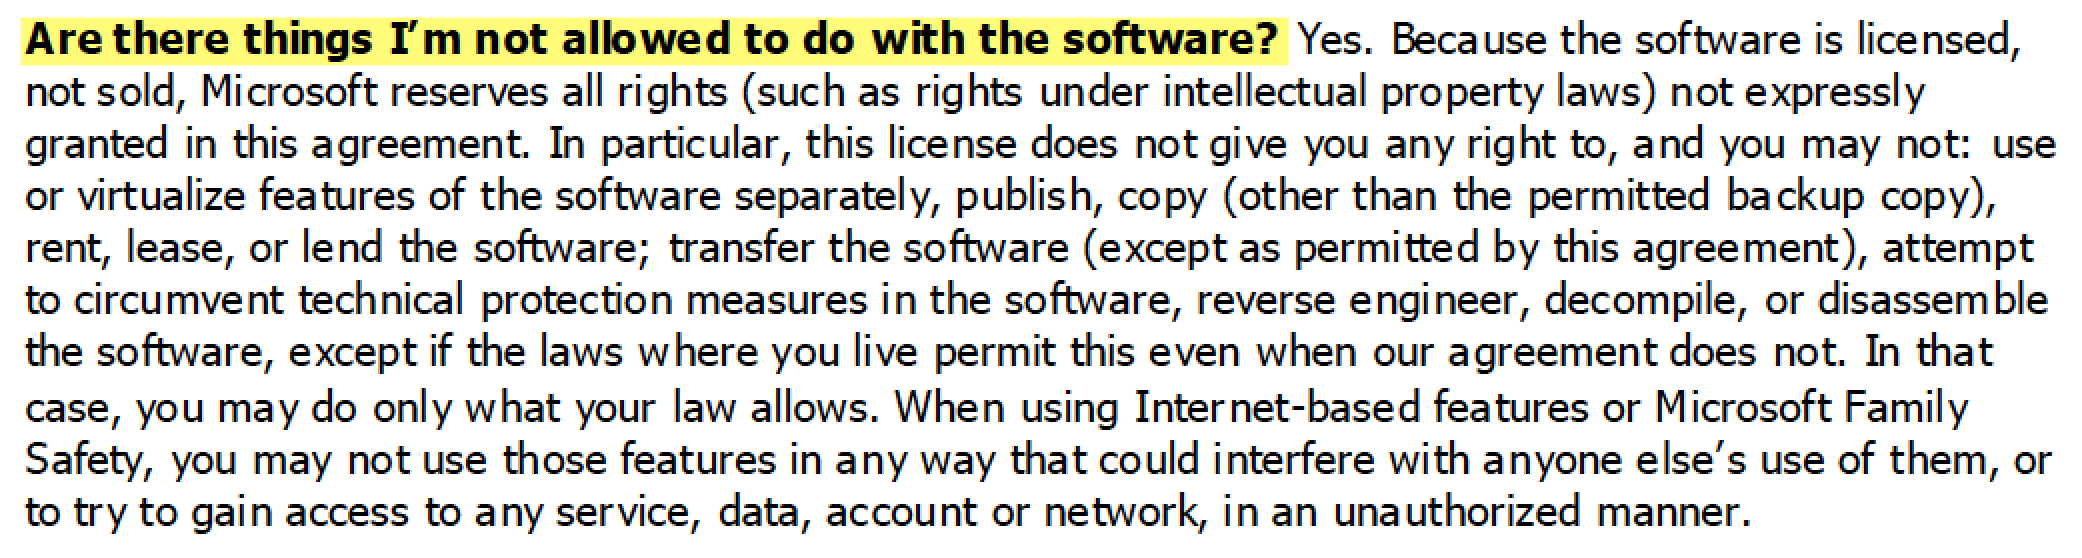
\includegraphics[scale=0.15]{windows_eula}

\end{frame}

\begin{frame}[fragile]{Apple macOS EULA}

\centering 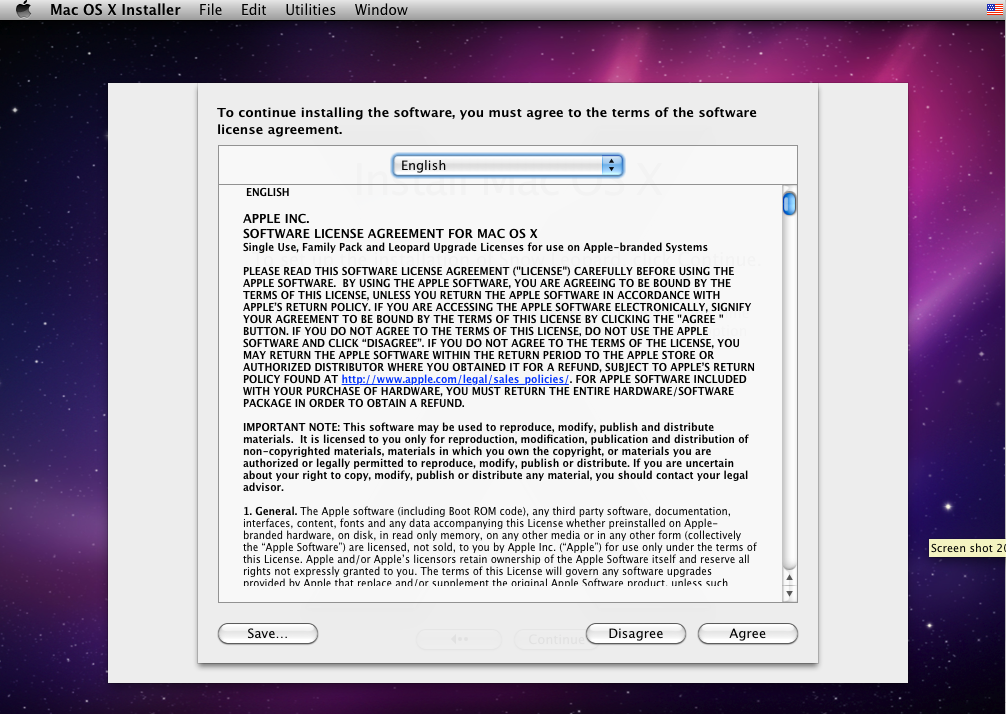
\includegraphics[scale=0.4]{apple_macos_eula}

\end{frame}

\begin{frame}[fragile]{Il software libero}

Un software è definito \textbf{software libero} quando concede alcune (o tutte) le libertà all'utente.

In Inglese si scrive \textbf{Free Software}, ma in questo caso \textit{free} non significa gratuito!

Un software che rilascia pubblicamente anche il codice sorgente è detto \textbf{Open Source}.

\end{frame}

\begin{frame}[fragile]{Le quattro libertà fondamentali}

\begin{itemize}
\item Libertà di eseguire il programma per qualsiasi scopo
\item \pause Libertà di studiare il programma e modificarlo
\item \pause Libertà di copiare il programma in modo da aiutare il prossimo
\item \pause Libertà di migliorare il programma e di distribuirne pubblicamente i miglioramenti, in modo tale che tutta la comunità ne tragga beneficio
\end{itemize}

\end{frame}

\begin{frame}[fragile]{Il progetto GNU}

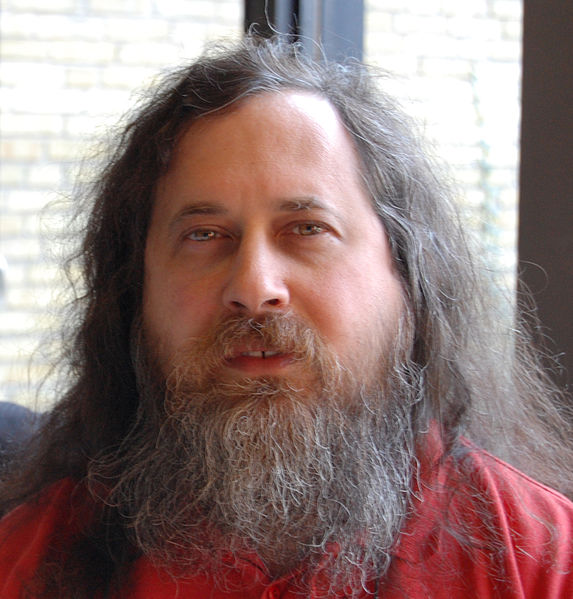
\includegraphics[scale=0.5]{stallman}

Nel 1984 nasce il progetto \textbf{GNU} ad opera di \textit{Richard Stallman}.

\textit{GNU} è un sistema operativo UNIX-like, ma libero (\textbf{Free Software}).

Il progetto \textit{GNU} aveva tante applicazioni, ma mancava di un kernel stabile.

\end{frame}

\begin{frame}[fragile]{Il lavoro di Linus Torvalds}
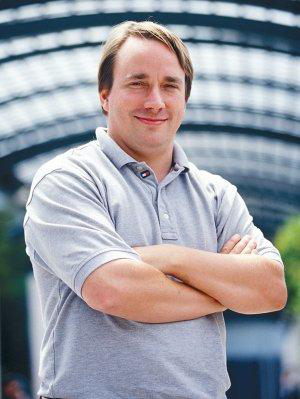
\includegraphics[scale=0.3]{linus}

Nel 1991 Linus Torvalds, uno studente finlandese, scrisse un kernel simile a quello del \textit{Minix} (il sistema operativo che aveva a scuola).

Rilasciò il suo kernel come software \textbf{Open Source}.

La comunità iniziò ad unire il kernel \textit{Linux} e gli strumenti di \textit{GNU} per formare \textbf{GNU/Linux}

\end{frame}

\section{GNU/Linux}

\begin{frame}[fragile]{Definizioni}
.
\end{frame}

\begin{frame}[fragile]{GNU/Linux nella vita quotidiana}
.
\end{frame}

\section{I Linux User Group}

\begin{frame}{LUG: Linux User Group}

I \textbf{Linux User Groups} sono delle associazioni (e/o semplici gruppi) di utilizzatori di software libero.

Lo scopo di formare un LUG è quello di diffondere l'uso di software libero (in particolare di \textbf{GNU/Linux}) attraverso iniziative, corsi ed eventi (come il \textit{Linux Day}).

\end{frame}

\begin{frame}[fragile]{LUG Latina}

Il LUG di Latina è un gruppo di persone con in comune l'interesse per il sistema operativo GNU/Linux rivolto a tutti gli utenti della provincia di Latina e zone limitrofe.

Nel tempo abbiamo curato diversi progetti, i più noti sono il recupero di hardware dismesso all'oratorio Don Bosco, ed i corsi di introduzione a GNU/Linux.

\begin{itemize}
\item \textbf{https://www.latinalug.it}
\item Telegram: \textbf{@latinalug} (oppure https://telegram.me/latinalug)
\end{itemize}

\end{frame}

\begin{frame}[standout]
  Questions?
\end{frame}

\begin{frame}{Conclusioni}

  \begin{center}\ccbysa\end{center}
  
  \center https://github.com/Enrico204/ld2017-intro

\end{frame}

\end{document}
